\chapter{Experiments}

\section{Method}

The benchmarks will compare the \texttt{Cata Sum}, \texttt{Generic Cata Sum} and \texttt{Incremental Cata Sum}. The Cata Sum is the simple function which traverses through the entire tree and sums all the values. The Generic Cata Sum is the initial Incremental Cata Sum, where all benchmarks start with an empty Map. And the Incremental Cata Sum, which already has a Map with intermediate results.

The benchmarks performed will measure the execution time and the memory usage. The execution time is in seconds and the memory usage will be the max-bytes-used. Every benchmark is implemented using the Haskell package \texttt{criterion}\cite{hackage2022criterion}. Criterion performs every benchmark multiple times within a time frame (default = 5s) to determine an average execution time. The criterion package is mainly focused on measuring performance, compared with measuring memory usage. It can apply a regression over the allocated bytes, however for these experiments it is not interesting how much memory is allocated, but how much memory is used. Therefore, for measuring the memory usage, the GHC profiler\cite*{ghc2022memoryprofiling} will be used to measure the max-bytes-used. Every benchmark will be individually executed, profiled and store its results in a file. 


The benchmarks will perform three types of updates: 
\begin{enumerate*}[label=(\arabic*)]
  \item Worst case: the lowest left leaf in the data structure is updated;
  \item Average case: the node halfway in the data structure is updated;
  \item Best case: removing the left size of the root node of the data structure.
\end{enumerate*} Additionally, every computation will be performed multiple times, depending on the amount of iterations given.

\section{Results}

\begin{itemize}
  \item Time/Memory
  \item Update
  \item Iterations
  \item Function
\end{itemize}



\subsection{Execution Time}

\begin{figure}[H]
  \begin{minipage}{.5\textwidth}
    \centering
    \includegraphics[width=\textwidth]{plots/run-0/time/Best/10/all_benchmarks.pdf}  
  \end{minipage}
  \begin{minipage}{.5\textwidth}
    \centering
    \includegraphics[width=\textwidth]{plots/run-0/time/Average/10/all_benchmarks.pdf}  
  \end{minipage}
\end{figure}

\begin{figure}[H]
  \centering
  \begin{minipage}[c]{.5\textwidth}
    \centering
    \includegraphics[width=\textwidth]{plots/run-0/time/Worst/10/all_benchmarks.pdf}  
  \end{minipage}
\end{figure}

\subsection{Memory Usage}

\begin{figure}[H]
  \begin{minipage}{.5\textwidth}
    \centering
    \includegraphics[width=\textwidth]{plots/run-0/memory/Best/10/all_benchmarks.pdf}  
  \end{minipage}
  \begin{minipage}{.5\textwidth}
    \centering
    \includegraphics[width=\textwidth]{plots/run-0/memory/Average/10/all_benchmarks.pdf}  
  \end{minipage}
\end{figure}

\begin{figure}[H]
  \centering
  \begin{minipage}[c]{.5\textwidth}
    \centering
    \includegraphics[width=\textwidth]{plots/run-0/memory/Worst/10/all_benchmarks.pdf}  
  \end{minipage}
\end{figure}

\subsection{Comparison Memory Strategies}